\documentclass{ximera}

%\usepackage{todonotes}

\newcommand{\todo}{}

\usepackage{esint} % for \oiint
\ifxake%%https://math.meta.stackexchange.com/questions/9973/how-do-you-render-a-closed-surface-double-integral
\renewcommand{\oiint}{{\large\bigcirc}\kern-1.56em\iint}
\fi


\graphicspath{
  {./}
  {ximeraTutorial/}
  {basicPhilosophy/}
  {functionsOfSeveralVariables/}
  {normalVectors/}
  {lagrangeMultipliers/}
  {vectorFields/}
  {greensTheorem/}
  {shapeOfThingsToCome/}
  {dotProducts/}
  {partialDerivativesAndTheGradientVector/}
  {../productAndQuotientRules/exercises/}
  {../normalVectors/exercisesParametricPlots/}
  {../continuityOfFunctionsOfSeveralVariables/exercises/}
  {../partialDerivativesAndTheGradientVector/exercises/}
  {../directionalDerivativeAndChainRule/exercises/}
  {../commonCoordinates/exercisesCylindricalCoordinates/}
  {../commonCoordinates/exercisesSphericalCoordinates/}
  {../greensTheorem/exercisesCurlAndLineIntegrals/}
  {../greensTheorem/exercisesDivergenceAndLineIntegrals/}
  {../shapeOfThingsToCome/exercisesDivergenceTheorem/}
  {../greensTheorem/}
  {../shapeOfThingsToCome/}
  {../separableDifferentialEquations/exercises/}
  {vectorFields/}
}

\newcommand{\mooculus}{\textsf{\textbf{MOOC}\textnormal{\textsf{ULUS}}}}

\usepackage{tkz-euclide}
\usepackage{tikz}
\usepackage{tikz-cd}
\usetikzlibrary{arrows}
\tikzset{>=stealth,commutative diagrams/.cd,
  arrow style=tikz,diagrams={>=stealth}} %% cool arrow head
\tikzset{shorten <>/.style={ shorten >=#1, shorten <=#1 } } %% allows shorter vectors

\usetikzlibrary{backgrounds} %% for boxes around graphs
\usetikzlibrary{shapes,positioning}  %% Clouds and stars
\usetikzlibrary{matrix} %% for matrix
\usepgfplotslibrary{polar} %% for polar plots
\usepgfplotslibrary{fillbetween} %% to shade area between curves in TikZ
%\usetkzobj{all}
\usepackage[makeroom]{cancel} %% for strike outs
%\usepackage{mathtools} %% for pretty underbrace % Breaks Ximera
%\usepackage{multicol}
\usepackage{pgffor} %% required for integral for loops



%% http://tex.stackexchange.com/questions/66490/drawing-a-tikz-arc-specifying-the-center
%% Draws beach ball
\tikzset{pics/carc/.style args={#1:#2:#3}{code={\draw[pic actions] (#1:#3) arc(#1:#2:#3);}}}



\usepackage{array}
\setlength{\extrarowheight}{+.1cm}
\newdimen\digitwidth
\settowidth\digitwidth{9}
\def\divrule#1#2{
\noalign{\moveright#1\digitwidth
\vbox{\hrule width#2\digitwidth}}}




% \newcommand{\RR}{\mathbb R}
% \newcommand{\R}{\mathbb R}
% \newcommand{\N}{\mathbb N}
% \newcommand{\Z}{\mathbb Z}

\newcommand{\sagemath}{\textsf{SageMath}}


%\renewcommand{\d}{\,d\!}
%\renewcommand{\d}{\mathop{}\!d}
%\newcommand{\dd}[2][]{\frac{\d #1}{\d #2}}
%\newcommand{\pp}[2][]{\frac{\partial #1}{\partial #2}}
% \renewcommand{\l}{\ell}
%\newcommand{\ddx}{\frac{d}{\d x}}

% \newcommand{\zeroOverZero}{\ensuremath{\boldsymbol{\tfrac{0}{0}}}}
%\newcommand{\inftyOverInfty}{\ensuremath{\boldsymbol{\tfrac{\infty}{\infty}}}}
%\newcommand{\zeroOverInfty}{\ensuremath{\boldsymbol{\tfrac{0}{\infty}}}}
%\newcommand{\zeroTimesInfty}{\ensuremath{\small\boldsymbol{0\cdot \infty}}}
%\newcommand{\inftyMinusInfty}{\ensuremath{\small\boldsymbol{\infty - \infty}}}
%\newcommand{\oneToInfty}{\ensuremath{\boldsymbol{1^\infty}}}
%\newcommand{\zeroToZero}{\ensuremath{\boldsymbol{0^0}}}
%\newcommand{\inftyToZero}{\ensuremath{\boldsymbol{\infty^0}}}



% \newcommand{\numOverZero}{\ensuremath{\boldsymbol{\tfrac{\#}{0}}}}
% \newcommand{\dfn}{\textbf}
% \newcommand{\unit}{\,\mathrm}
% \newcommand{\unit}{\mathop{}\!\mathrm}
% \newcommand{\eval}[1]{\bigg[ #1 \bigg]}
% \newcommand{\seq}[1]{\left( #1 \right)}
% \renewcommand{\epsilon}{\varepsilon}
% \renewcommand{\phi}{\varphi}


% \renewcommand{\iff}{\Leftrightarrow}

% \DeclareMathOperator{\arccot}{arccot}
% \DeclareMathOperator{\arcsec}{arcsec}
% \DeclareMathOperator{\arccsc}{arccsc}
% \DeclareMathOperator{\si}{Si}
% \DeclareMathOperator{\scal}{scal}
% \DeclareMathOperator{\sign}{sign}


%% \newcommand{\tightoverset}[2]{% for arrow vec
%%   \mathop{#2}\limits^{\vbox to -.5ex{\kern-0.75ex\hbox{$#1$}\vss}}}
% \newcommand{\arrowvec}[1]{{\overset{\rightharpoonup}{#1}}}
% \renewcommand{\vec}[1]{\arrowvec{\mathbf{#1}}}
% \renewcommand{\vec}[1]{{\overset{\boldsymbol{\rightharpoonup}}{\mathbf{#1}}}}

% \newcommand{\point}[1]{\left(#1\right)} %this allows \vector{ to be changed to \vector{ with a quick find and replace
% \newcommand{\pt}[1]{\mathbf{#1}} %this allows \vec{ to be changed to \vec{ with a quick find and replace
% \newcommand{\Lim}[2]{\lim_{\point{#1} \to \point{#2}}} %Bart, I changed this to point since I want to use it.  It runs through both of the exercise and exerciseE files in limits section, which is why it was in each document to start with.

% \DeclareMathOperator{\proj}{\mathbf{proj}}
% \newcommand{\veci}{{\boldsymbol{\hat{\imath}}}}
% \newcommand{\vecj}{{\boldsymbol{\hat{\jmath}}}}
% \newcommand{\veck}{{\boldsymbol{\hat{k}}}}
% \newcommand{\vecl}{\vec{\boldsymbol{\l}}}
% \newcommand{\uvec}[1]{\mathbf{\hat{#1}}}
% \newcommand{\utan}{\mathbf{\hat{t}}}
% \newcommand{\unormal}{\mathbf{\hat{n}}}
% \newcommand{\ubinormal}{\mathbf{\hat{b}}}

% \newcommand{\dotp}{\bullet}
% \newcommand{\cross}{\boldsymbol\times}
% \newcommand{\grad}{\boldsymbol\nabla}
% \newcommand{\divergence}{\grad\dotp}
% \newcommand{\curl}{\grad\cross}
%\DeclareMathOperator{\divergence}{divergence}
%\DeclareMathOperator{\curl}[1]{\grad\cross #1}
% \newcommand{\lto}{\mathop{\longrightarrow\,}\limits}

% \renewcommand{\bar}{\overline}

\colorlet{textColor}{black}
\colorlet{background}{white}
\colorlet{penColor}{blue!50!black} % Color of a curve in a plot
\colorlet{penColor2}{red!50!black}% Color of a curve in a plot
\colorlet{penColor3}{red!50!blue} % Color of a curve in a plot
\colorlet{penColor4}{green!50!black} % Color of a curve in a plot
\colorlet{penColor5}{orange!80!black} % Color of a curve in a plot
\colorlet{penColor6}{yellow!70!black} % Color of a curve in a plot
\colorlet{fill1}{penColor!20} % Color of fill in a plot
\colorlet{fill2}{penColor2!20} % Color of fill in a plot
\colorlet{fillp}{fill1} % Color of positive area
\colorlet{filln}{penColor2!20} % Color of negative area
\colorlet{fill3}{penColor3!20} % Fill
\colorlet{fill4}{penColor4!20} % Fill
\colorlet{fill5}{penColor5!20} % Fill
\colorlet{gridColor}{gray!50} % Color of grid in a plot

\newcommand{\surfaceColor}{violet}
\newcommand{\surfaceColorTwo}{redyellow}
\newcommand{\sliceColor}{greenyellow}




\pgfmathdeclarefunction{gauss}{2}{% gives gaussian
  \pgfmathparse{1/(#2*sqrt(2*pi))*exp(-((x-#1)^2)/(2*#2^2))}%
}


%%%%%%%%%%%%%
%% Vectors
%%%%%%%%%%%%%

%% Simple horiz vectors
\renewcommand{\vector}[1]{\left\langle #1\right\rangle}


%% %% Complex Horiz Vectors with angle brackets
%% \makeatletter
%% \renewcommand{\vector}[2][ , ]{\left\langle%
%%   \def\nextitem{\def\nextitem{#1}}%
%%   \@for \el:=#2\do{\nextitem\el}\right\rangle%
%% }
%% \makeatother

%% %% Vertical Vectors
%% \def\vector#1{\begin{bmatrix}\vecListA#1,,\end{bmatrix}}
%% \def\vecListA#1,{\if,#1,\else #1\cr \expandafter \vecListA \fi}

%%%%%%%%%%%%%
%% End of vectors
%%%%%%%%%%%%%

%\newcommand{\fullwidth}{}
%\newcommand{\normalwidth}{}



%% makes a snazzy t-chart for evaluating functions
%\newenvironment{tchart}{\rowcolors{2}{}{background!90!textColor}\array}{\endarray}

%%This is to help with formatting on future title pages.
\newenvironment{sectionOutcomes}{}{}



%% Flowchart stuff
%\tikzstyle{startstop} = [rectangle, rounded corners, minimum width=3cm, minimum height=1cm,text centered, draw=black]
%\tikzstyle{question} = [rectangle, minimum width=3cm, minimum height=1cm, text centered, draw=black]
%\tikzstyle{decision} = [trapezium, trapezium left angle=70, trapezium right angle=110, minimum width=3cm, minimum height=1cm, text centered, draw=black]
%\tikzstyle{question} = [rectangle, rounded corners, minimum width=3cm, minimum height=1cm,text centered, draw=black]
%\tikzstyle{process} = [rectangle, minimum width=3cm, minimum height=1cm, text centered, draw=black]
%\tikzstyle{decision} = [trapezium, trapezium left angle=70, trapezium right angle=110, minimum width=3cm, minimum height=1cm, text centered, draw=black]


\title{Sine and Cosine}

\begin{document}

\begin{abstract}
derivatives
\end{abstract}
\maketitle








In the graph below, 

\begin{itemize}
\item the measurement for the angle $\theta$ is plotted horizontally
\item $\sin(\theta)$ is the green thicker curve
\item the blue line is a tangent line to $\sin(\theta)$
\item the slope of the tangent line is a number and is plotted as the red dot
\end{itemize}

As you move long the $\sin(\theta)$ curve, the slope of the tangent line follows the red $\cos(\theta)$ curve.








\begin{center}
\desmos{ysuoxzmvfq}{400}{300}
\end{center}



The values of $\cos(\theta)$ measure the instantaneous rate of change of $\sin(\theta)$.



\begin{theorem}  \textbf{\textcolor{green!50!black}{Derivative of $\sin(\theta)$}}

\begin{center}
$\cos(\theta)$ is the derivative of $\sin(\theta)$.  

$\cos(\theta)$ measures the instantaneous rate of change of $\sin(\theta)$.  
\end{center}


\[
\frac{d}{d\theta} \sin(\theta) = \cos(\theta)
\]

\end{theorem}















In the graph below, 

\begin{itemize}
\item the measurement for the angle $\theta$ is plotted horizontally
\item $\cos(\theta)$ is the blue curve
\item the line is a tangent line to $\cos(\theta)$
\item the slope of the tangent line is a number and is plotted as the red dot
\end{itemize}

As you move long the $\cos(\theta)$ curve, the slope of the tangent line follows the dotted $-\sin(\theta)$ curve.



\begin{center}
\desmos{mushid6bj8}{400}{300}
\end{center}



The values of $-\sin(\theta)$ measure the instantaneous rate of change of $\cos(\theta)$.



\begin{theorem}  \textbf{\textcolor{green!50!black}{Derivative of $\cos(\theta)$}}

\begin{center}
$-\sin(\theta)$ is the derivative of $\cos(\theta)$. 

$-\sin(\theta)$ measures the instantaneous rate of change of $\cos(\theta)$. 
\end{center}


\[
\frac{d}{d\theta} \cos(\theta) = -\sin(\theta)
\]


\end{theorem}







We use these two facts as our algebraic reasoning for the behavior of $\sin(\theta)$ and $\cos(\theta)$.




\begin{example}



$f(t) = \sin(t)$ is decreasing at $t=\frac{2\pi}{3}$, because $\cos\left( \frac{2\pi}{3} \right) < 0$ \\


$g(t) = \cos(t)$ is decreasing at $t=\frac{\pi}{4}$, because $-\sin\left( \frac{\pi}{4} \right) < 0$

\end{example}

















\subsection*{Shifts}




If the graph $y = \sin(t)$ is vertically shifted to $y = \sin(t)+C$, then the shape of the graph does not change. The graph just rigidly moves up. Therefore, the slopes of the tangent lines at the shifted points are the same as for $y = \sin(t)$ .



\begin{observation} \textbf{\textcolor{purple!85!blue}{Vertical Shifts}}  \\

Shifting a graph vertically doesn't change the shape.  It just repositions the graph.  Therefore, all of the slopes of the tangents lines stay the same. \\



$\blacktriangleright$ The derivative of $\sin(t)+C$ is $\cos(t)$. \\

$\blacktriangleright$ The derivative of $\cos(t)+C$ is $-\sin(t)$. \\

\end{observation}


\begin{notation}

\[
\frac{d}{d\theta} (\sin(\theta) + C) = \cos(\theta)
\]

\[
\frac{d}{d\theta} (\cos(\theta) + C) = -\sin(\theta)
\]

\end{notation}


If the graph $y = \sin(t)$ is horizontally shifted to $y = \sin(t - B)$, then the shape of the graph does not change. The whole graph is just picked up and set down at a new location. Therefore, the slopes of the tangent lines at the shifted points don't change.



\begin{observation} \textbf{\textcolor{purple!85!blue}{Horizontal Shifts}} \\

$\blacktriangleright$ The derivative of $\sin(t - B)$ is $\cos(t - B)$. \\

$\blacktriangleright$ The derivative of $\cos(t - B)$ is $-\sin(t - B)$. \\

\end{observation}


\begin{notation}

\[
\frac{d}{d\theta} \sin(\theta - B) = \cos(\theta - B)
\]

\[
\frac{d}{d\theta} \cos(\theta - B) = -\sin(\theta - B)
\]

\end{notation}













\subsection*{Stretching}


Suppose you have a line $L$ with slope $m$. \\

Let $(x_1, y_1)$ and $(x_2, y_2)$ be any two distinct points on $L$. \\

Then, we have


\[
m = \frac{y_2 - y_1}{x_2 - x_1}
\]






Now, suppose we stretch the line vertically by a factor of $k$.  That means that all of the points change from $(a, b)$ to $(a, k \cdot b)$

Then, the new slope, $M$, is 



\[
M = \frac{k \cdot y_2 - k \cdot y_1}{x_2 - x_1} = \frac{k \cdot (y_2 - y_1)}{x_2 - x_1} = k \cdot \frac{y_2 - y_1}{x_2 - x_1} = k \cdot m
\]


If you stretch the graph of a function vertically by a factor of $k$, then you also stretch all of the tangent lines by the same factor.


\begin{observation} \textbf{\textcolor{purple!85!blue}{Vertical Stretching}}   \\

$\blacktriangleright$ The derivative of $k \cdot \sin(t)$ is $k \cdot \cos(t)$. \\

$\blacktriangleright$ The derivative of $k \cdot \cos(t)$ is $-k \cdot \sin(t)$. \\

\end{observation}




\begin{notation}

\[
\frac{d}{d\theta} k \, \sin(\theta) = k \, \cos(\theta)
\]

\[
\frac{d}{d\theta} k \, \cos(\theta) = -k \, \sin(\theta)
\]

\end{notation}








Let's put all of this together.







\begin{theorem} \textbf{\textcolor{green!50!black}{Derivatives}}  \\

$\blacktriangleright$ The derivative of \textbf{\textcolor{purple!85!blue}{$A \, \sin(t - B) + C$}} is \textbf{\textcolor{blue!55!black}{$A \, \cos(t - B)$}}. \\

$\blacktriangleright$ The derivative of \textbf{\textcolor{purple!85!blue}{$A \, \cos(t - B) + C$}} is \textbf{\textcolor{blue!55!black}{$-A \, \sin(t - B)$}}. \\

\end{theorem}






\begin{notation}

\[
\frac{d}{d\theta} (A \, \sin(\theta - B) + C) = A \, \cos(\theta - B)
\]

\[
\frac{d}{d\theta} (A \, \cos(\theta - B) + C) = -A \, \sin(\theta - B)
\]

\end{notation}










\begin{example}


What is the slope of the tangent line to the graph of $H(t) = -2 \sin\left( t - \frac{\pi}{6} \right) + 3$ at $\left( \frac{5 \pi}{6}, 3-\sqrt{3} \right)$?




\begin{image}
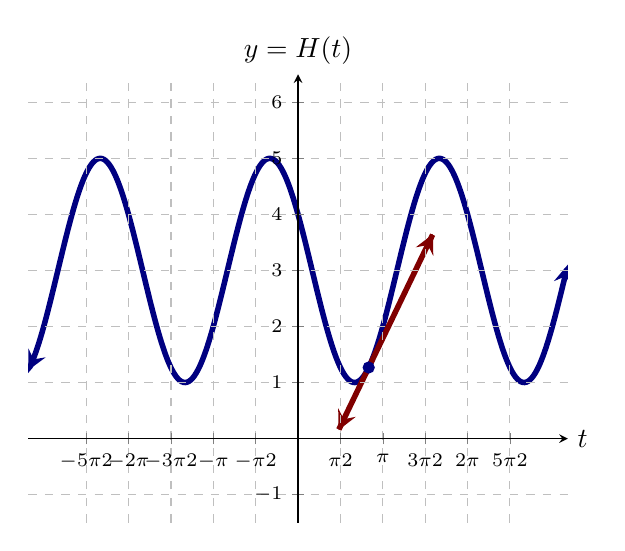
\begin{tikzpicture}
  \begin{axis}[
            domain=-10:10, ymax=6.5, xmax=10, ymin=-1.5, xmin=-10,
            axis lines =center, xlabel={$t$}, ylabel={$y = H(t)$}, grid = major, grid style={dashed},
            ytick={-1,1,2,3,4,5,6},
            xtick={-7.85, -6.28, -4.71, -3.14, -1.57, 0, 1.57, 3.142, 4.71, 6.28, 7.85},
            xticklabels={$-\tfrac{5\pi}{2}$,$-2\pi$,$-\tfrac{3\pi}{2}$,$-\pi$, $-\tfrac{\pi}{2}$, $0$, $\tfrac{\pi}{2}$, $\pi$, $\tfrac{3\pi}{2}$, $2\pi$, $\tfrac{5\pi}{2}$},
            yticklabels={$-1$,$1$,$2$,$3$,$4$,$5$,$6$}, 
            ticklabel style={font=\scriptsize},
            every axis y label/.style={at=(current axis.above origin),anchor=south},
            every axis x label/.style={at=(current axis.right of origin),anchor=west},
            axis on top
          ]
          

            \addplot [line width=2, penColor, smooth,samples=300,domain=(-10:10),<->] {-2 * sin(deg(x - 0.523)) + 3};
            %\addplot [line width=2, penColor2, smooth,samples=300,domain=(-10:10),<->] {cos(deg(x)};

			\addplot [line width=2, penColor2, smooth,samples=300,domain=(1.5:5),<->] { (x-2.618) + 1.268};

            \addplot [color=penColor,only marks,mark=*] coordinates{(2.618,1.2679)};



  \end{axis}
\end{tikzpicture}
\end{image}



\begin{explanation}



The derivative of $f(t) = -2 \sin\left( t - \frac{\pi}{6} \right) + 3$ is $f'(t) = -2 \cos\left( t - \frac{\pi}{6} \right)$.



\[ f'\left( \frac{5 \pi}{6} \right) = -2 \cos\left( \frac{5 \pi}{6} - \frac{\pi}{6} \right) = -2 \cos\left( \frac{2 \pi}{3} \right)  = -2 \cdot -\frac{1}{2} = 1\]


The slope of the tangent line is $1$.

\end{explanation}

\end{example}












\begin{example}


Let $G(x) = 3 \cos\left( x +\frac{\pi}{4} \right) - 1$.

Where does the graph of $y = G(x)$ have horizontal tangent lines?




\begin{image}
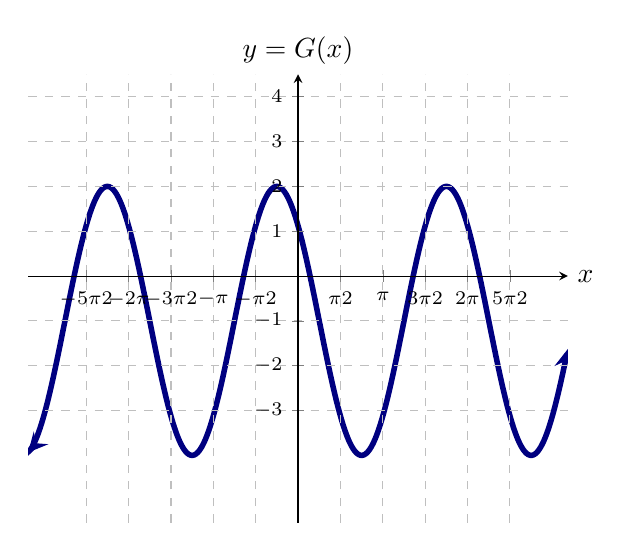
\begin{tikzpicture}
  \begin{axis}[
            domain=-10:10, ymax=4.5, xmax=10, ymin=-5.5, xmin=-10,
            axis lines =center, xlabel={$x$}, ylabel={$y = G(x)$}, grid = major, grid style={dashed},
            ytick={-3,-2,-1,1,2,3,4,5},
            xtick={-7.85, -6.28, -4.71, -3.14, -1.57, 0, 1.57, 3.142, 4.71, 6.28, 7.85},
            xticklabels={$-\tfrac{5\pi}{2}$,$-2\pi$,$-\tfrac{3\pi}{2}$,$-\pi$, $-\tfrac{\pi}{2}$, $0$, $\tfrac{\pi}{2}$, $\pi$, $\tfrac{3\pi}{2}$, $2\pi$, $\tfrac{5\pi}{2}$},
            yticklabels={$-3$,$-2$,$-1$,$1$,$2$,$3$,$4$,$5$,$6$}, 
            ticklabel style={font=\scriptsize},
            every axis y label/.style={at=(current axis.above origin),anchor=south},
            every axis x label/.style={at=(current axis.right of origin),anchor=west},
            axis on top
          ]
          

            \addplot [line width=2, penColor, smooth,samples=300,domain=(-10:10),<->] {3 * cos(deg(x + 0.785)) - 1};
            %\addplot [line width=2, penColor2, smooth,samples=300,domain=(-10:10),<->] {cos(deg(x)};

			%\addplot [line width=2, penColor2, smooth,samples=300,domain=(1.5:5),<->] { (x-2.618) + 1.268};

            %\addplot [color=penColor,only marks,mark=*] coordinates{(2.618,1.2679)};



  \end{axis}
\end{tikzpicture}
\end{image}



We have two approaches:

\begin{explanation} \textbf{\textcolor{blue!55!black}{Maximums and Minimums}}  \\

The horizontal tangent lines occur at points which correspond to maximums and minimums of cosine.  


$\blacktriangleright$ Maximums of cosine functions occur when the inside of the function equals $2 k \pi$ where $k \in \mathbb{Z}$.


\[
x + \frac{\pi}{4} = 2 k \pi
\]

\[
x = 2 k \pi - \frac{\pi}{4} = \frac{8 k \pi}{4} - \frac{\pi}{4} = \frac{(8k - 1)\pi}{4}
\]




$\blacktriangleright$ Minimums of cosine functions occur when the inside of the function equals $(2 k + 1) \pi$ where $k \in \mathbb{Z}$.


\[
x + \frac{\pi}{4} = (2 k + 1) \pi
\]

\[
x = (2 k + 1) \pi - \frac{\pi}{4} = \frac{4(2 k + 1) \pi}{4} - \frac{\pi}{4} = \frac{(8k + 3)\pi}{4}
\]


\end{explanation}








\begin{explanation} \textbf{\textcolor{blue!55!black}{Critical Numbers}} \\


The horizontal tangent lines occur at points which correspond to where the derivative equals $0$.  






The derivative of $G(x) = 3 \cos\left( x + \frac{\pi}{4} \right) - 1$ is $G'(x) = -3 \sin\left( x + \frac{\pi}{4} \right)$.


The sine function equals $0$ at $k \pi$ where $k \in \mathbb{Z}$.



\[
x + \frac{\pi}{4} =  k \pi
\]


\[
x  =    k \pi - \frac{\pi}{4} =  \frac{4 k \pi}{4} - \frac{\pi}{4} = \frac{(4k - 1)\pi}{4}
\]









\end{explanation}



Did these two methods give the same set of domain numbers? \\



\[
\frac{(8k - 1)\pi}{4} :  \cdots \frac{-17\pi}{4}, \frac{-9\pi}{4}, \frac{-\pi}{4}, \frac{7\pi}{4} \cdots
\]

\[
\frac{(8k + 3)\pi}{4} :  \cdots \frac{-13\pi}{4}, \frac{-5\pi}{4}, \frac{3\pi}{4}, \frac{11\pi}{4} \cdots
\]


\[
\frac{(4k - 1)\pi}{4} :  \cdots \frac{-9\pi}{4}, \frac{-5\pi}{4}, \frac{-\pi}{4}, \frac{3\pi}{4} \cdots
\]



Yep.  They are generating the same list.


\end{example}
































\subsection*{Notation}











Calculus is the story about the very small.  We talk about quantities that are smaller than any specific number.  ``Infinitesimal'' is the mathematics word for these quantities. Since infinitesimals are smaller than any of our numbers, we can't describe them with our numbers.  \\

The language of \textbf{limits} is our way of discussing the concepts of infinitesimals.  


For rates of change, the infinitesimal story involves instantaneous rate of change.  Our tool for measuring this type of change comparison is called the \textbf{derivative}.

We have a couple of ways of representing the derivative of a function. \\


$\blacktriangleright$  \textbf{\textcolor{purple!85!blue}{Prime Notation}}


Suppose $f$ is the name of a function.

The derivative of $f$ is a new function and it is denoted as \textbf{\textcolor{purple!85!blue}{$f'$}}.

The little ``tick mark'' in the exponent position is called the \textbf{\textcolor{purple!85!blue}{prime sign}}.


$f'$ is pronounced as ``f prime''.


The derivative measures the change in the function values compared to changes in the domain values - at the infinitesimal level. It may not seem like it now, but, this is (will be) straightforward for most situations.  However, we often encounter situations where our function representation involves parameters, like


\[
f = A \sin(t - B) + C
\]

Which symbol is representing the domain?


\[
f(A)   \, \text{ or } \, f(t)   \, \text{ or } \, f(B)   \, \text{ or } \, f(C)   
\]


Or, more to the point, functions of more than one variable:


\[
f(x, y) = \sin(2x - 3y)
\]

To which variable is $f'$ referring? \\






It can be confusing at times.  Therefore, we have an alternative notation for derivatives to clear up the confusion.



$\blacktriangleright$  \textbf{\textcolor{purple!85!blue}{Leibniz Notation}}


\textbf{Gottfried Leibniz} was a German mathematician who was investigating the concepts of Calculus at the same time as Newton.  While Newton developed his ``dot'' notation for derivative, Leibniz invented a more useful notation.


The derivative of $f$ with respect to $x$ is represented as $\frac{df}{dx}$. \\

$\frac{df}{dx}$ is pronounced as ``dfdx''.  It looks like a fraction, but it isn't.


``with respect to $x$'' means $x$ is representing the domain for rate measurment purposes. 



\begin{notation}


Just like with other mathematical notation, we allow useful modifications to this notation.



As the symbol $\frac{df}{dx}$ shows, the function should be on top next to the $d$.    We should write $\frac{d sin(x)}{dx}$.  However, if the formula for the function gets long, then it becomes difficult to read the notation. For instance,

\[
\frac{d (\sin(3x^2+1)\ln(\cos(5x+7))e^{\tan(4x)})}{dx}
\]


Therefore, it is sometimes clearer if the function is placed to the right of the differentiation notation:




\[
\frac{d}{dx} \, (\sin(3x^2+1)\ln(\cos(5x+7))e^{\tan(4x)})
\]






\end{notation}




Calculus will dive deep into all of this notation. \\

We are just introducing it and bringing it into our vocabulary, so that we can recognize and follow the symbols in Calculus, because it tends to go by fast there.






















\begin{center}
\textbf{\textcolor{green!50!black}{ooooo-=-=-=-ooOoo-=-=-=-ooooo}} \\

more examples can be found by following this link\\ \link[More Examples of Rates of Change]{https://ximera.osu.edu/csccmathematics/precalculus2/precalculus2/rateOfChange/examples/exampleList}

\end{center}

\end{document}
